\section{Experiments}
\label{sec:exp}

\subsection{Experimental Setup}
All experiments were run in Intel Core i5-2310 CPU @ 2.90GHz machines
with 8GB of RAM memory running Linux Mint 13. To solve the integer 
programming problems we have used the GLPK LP/MIP solver,
version 4.43. To facilitate the job distribution we have used the HTCondor framework.

\subsection{Instance Generator}
To create the instances for our analysis we have implemented a random instance generator.
We have tried to mimic the characteristics of real-world actions supplied by the local EDCO.
Algorithm~\ref{alg:gen} defines the pseudo-code of the random instance generator.

\begin{algorithm}[H]
\begin{algorithmic}[1]
\Function{Generator}{Correlation factor $\alpha$, Number of years $M$, Number of actions $N$}
\State \label{line:gen1} $BudgetMean \gets UniformRandom(700,800)$
\State $BudgetVariance \gets UniformRandom(10,20)$
\For{$i=1 \to M$}
  \State $o_{i1} \gets GaussRandom(BudgetMean,$ $BudgetVariance)$
\EndFor \label{line:gen2}
\For{$j=1 \to N$}\label{line:gen3}
  \State $c_{j1} \gets \label{line:min} Min(Min(o), UniformRandom(1,100))$
\EndFor
\For{$j=1 \to N$}
  \State \label{line:market} $ m_j = 2 Sum(o) / M c_{j1}$
\EndFor \label{line:gen4}

\For{$j=1 \to N$} \label{line:W1}
  \For{$i=1 \to M$}
    \State $W{ji} \gets UniformRandom(0,1)$
  \EndFor
  \State $W{j} \gets ReverSort(W{j})$
\EndFor

\For{$j=1 \to N$}
  \State $s \gets 0$
  \For{$i=1 \to M$}
    \State $s \gets s + W_{ji}$
  \EndFor
  \For{$i=1 \to M$}
    \State $W_{ji} \gets W_{ji}/s$
  \EndFor
\EndFor  \label{line:W2}

\For{$i=1 \to M$} \label{line:e1}
  \For{$j=1 \to N$}
      \State \label{line:en} $e_{j,k} \gets Max(0, Abs((1-\alpha)c_{j1} W_{ji} + UniformRandom(-100,100)\alpha))$
  \EndFor
\EndFor \label{line:e2}
\EndFunction
\end{algorithmic}
\caption{Random instance generator}
\label{alg:gen}
\end{algorithm}

Lines \ref{line:gen1} to \ref{line:gen2} present the generation of the yearly budgets from a Gaussian
distribution (function $GaussRandom(mean, variance)$) that in turn has its variance and mean draw 
from a uniform distribution of fixed parameters (function $UniformRandom(Lower\,bound,\,Upper\,bound)$).
The parameters were inspired by real-world actions, given by the local EDCO.

Lines \ref{line:gen3} to \ref{line:gen4} generate the cost and market of each action, the cost comes from
an uniform random distribution with fixed parameters. Note that in line \ref{line:min} we
use the $Min$ function to guarantee that the action may performed at least one time. Line \ref{line:market}
defines the market of each action as a function of the total budget over all years ($Sum(o)$) and the
cost of the action. That is, the cheapest the action the larger the market.

Lines \ref{line:W1} to \ref{line:W2} are used to build the reverse-ordered normalized weight matrix that is used to 
build the recuperation over the years. After line \ref{line:W2}, the $j$-th line of matrix $W$ will contain
a vector of values that add to 1 and are reversely ordered, e.g., a possible $W$ matrix for 3 years and 4 actions
could be:
\[ W = \left( \begin{array}{ccc}
0.7 & 0.2 & 0.1 \\
0.8 & 0.1 & 0.1 \\
0.6 & 0.2 & 0.2 \\
1.0 & 0.0 & 0.0 \end{array} \right).\] 

Finally from lines \ref{line:e1} to \ref{line:e2} the energy recuperation values are defined for each action
and each year. In line \ref{line:en} we may see that the use of matrix $W$ guarantees that the energy recuperation has an decreasing tendency
over the years. In this line we also present the use of the correlation parameter $\alpha$, $\alpha \in [0,1]$,
the closest alpha is to one, the weaker the correlation.

The generator was implemented in the Python programming language and it is available at \todo[inline]{URL}.

\subsection{Time Analysis}

\subsubsection{The Impact of Correlation}
Literature on the knapsack problem states that a strong correlation between the value of the item
and its weight greatly affects the complexity of the problem. In fact, it has been demonstrated
that a weak correlation among weight and value renders the complexity of the problem polynomial
on the size of the problem~\ref{???}.

To test if this phenomena repeats itself in our problem when using the exact algorithm, we have tested the values $[0.0, 0.1, 1.0]$ for $\alpha$,
the parameter that control the randomness of the value of the action, in a number of problem sizes. When $\alpha$ is 0,
there is a strong correlation between the cost of the action and its energy return, that is,
the more expensive the action, the more effective it is. When $\alpha$ is 1 there is no correlation
between the value of the actions and its effectiveness. When $\alpha$ is 0.1, there is a weak correlation between cost and value.
The alpha values of 0.0, 0.1 and 1.0 are equivalent to the the following classes of problems defined by \cite{Pisinger05whereare} (respectively): 
\textit{subset sum instances, weakly correlated instances and uncorrelated instances.}

Figures~\ref{fig:time1} to~\ref{fig:time3} display the amount of instances that successfully executed in less than 1 hour,
given value of alpha. For each cell of the figure the exact algorithm was run 10 times using random instances of the problem.
The closer to black, the greater the amount of successful runs. White cells represent problem sizes that contains 0 successful
runs.  From the figures it is clear that the bigger the problem the likely it is that it will take more than 1 hour, also, it may be observed that the more
correlated the cost is with the profit, the harder the problems seems to be, as predicted by the literature.

\begin{figure}
\centering
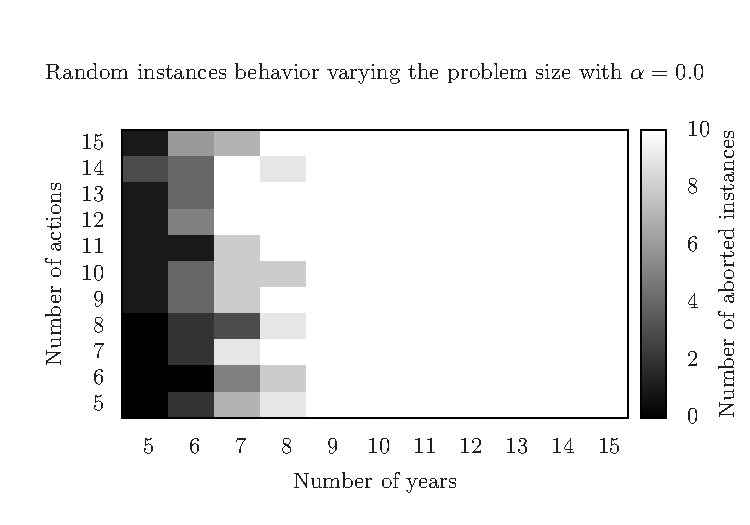
\includegraphics[scale=0.73, trim=1cm 0 0 0]{figs/very_hard.pdf}
\caption{Strong correlation between cost and profit.}
\label{fig:time1}
\end{figure}

\begin{figure}
\centering
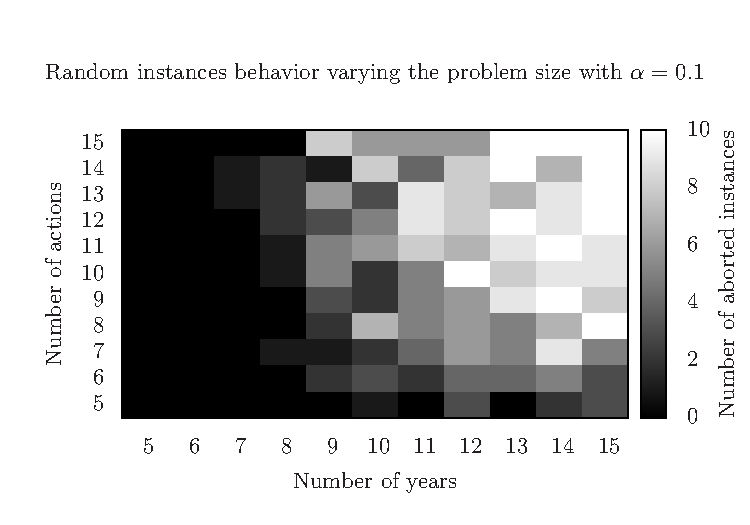
\includegraphics[scale=0.73, trim=1cm 0 0 0]{figs/hard.pdf}
\caption{Weak correlation between cost and profit.}
\label{fig:time2}
\end{figure}

\begin{figure}
\centering
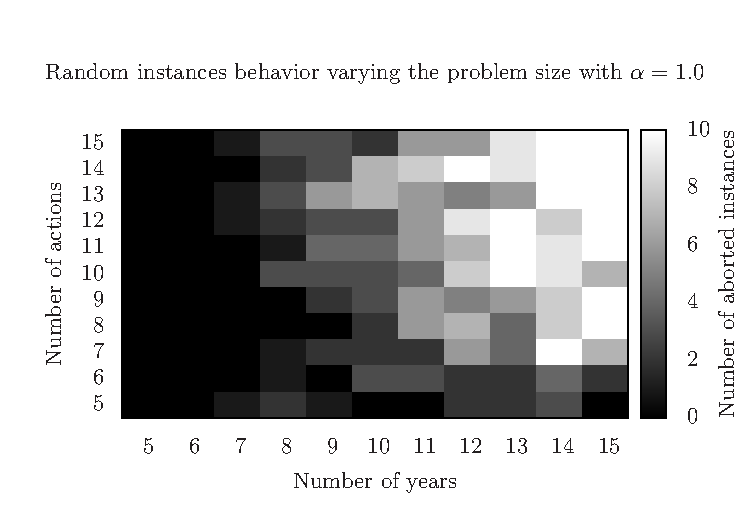
\includegraphics[scale=0.73 ,trim=1cm 0 0 0]{figs/easy.pdf}
\caption{No correlation between cost and profit.}
\label{fig:time3}
\end{figure}

To further investigate the impact of the value of alpha in the overall run time we have selected a cell of the
figure, namely $5\times5$ and varied the value of alpha to analyse its impact in the running time more precisely.
Figure~\ref{fig:alpha_5_5} displays the impact of the value of $alpha$ in the total running time of the instances for a
problem size of $5\times5$. The line observed in this figure suggests that the complexity of the problem 
decreases linearly as the correlation increases.

\begin{figure}
\centering
\missingfigure[figwidth=8cm]{}
\caption{Analysis of the running time varying the value of $\alpha$.}
\label{fig:alpha_5_5}
\end{figure}

Figures~\ref{fig:alpha_10_5} to \ref{fig:alpha_10_10} display the results for other problem sizes,
it can be observed that the dimension of the problem does not alter the overall linear characteristic observed in
the smaller instance. We find this result intriguing and counter-intuitive, since the existence of obviously
preferable actions should take the problem easier to solve, not the contrary.

\begin{figure}
\centering
\missingfigure[figwidth=8cm]{}
\caption{Blah blah blah}
\label{fig:alpha_10_5}
\end{figure}

\begin{figure}
\centering
\missingfigure[figwidth=8cm]{}
\caption{Blah blah blah}
\label{fig:alpha_5_10}
\end{figure}

\begin{figure}
\centering
\missingfigure[figwidth=8cm]{}
\caption{Blah blah blah}
\label{fig:alpha_10_10}
\end{figure}

\subsection{Solution Analysis - Small Instances}

In this subsection we compare the solution quality of the implemented heuristics
in the set of small instances, there is, the instances in which the exact algorithm
found the optimal solution in less then two hours. We have also limited the running time
of the meta heuristics in two hours.

Figures~\ref{fig:mh1_1} to \ref{fig:mh2_3} display the average ratio between the optimal solution (when available) 
and the solution found by the meta-heuristics. White cells represent problem sizes with no
optimal solution found. Small relative differences are darker than large diferences.

\begin{figure}
\centering
%\missingfigure[figwidth=8cm]{}
%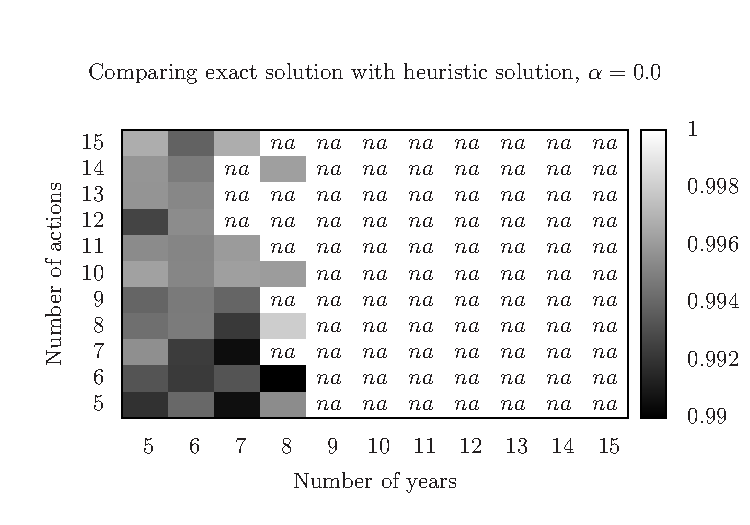
\includegraphics[scale=0.73, trim=1cm 0 0 0]{figs/comp_very_hard.pdf}
\caption{Comparison between the optimal solution (when available) 
and the solution by the meta-heuristics for $\alpha=0.0$.}
\label{fig:mh1_1}
\end{figure}

\begin{figure}
\centering
%\missingfigure[figwidth=8cm]{}
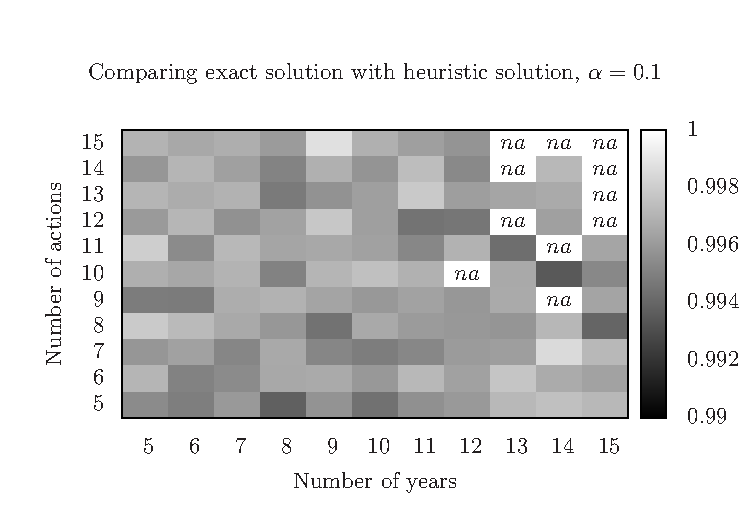
\includegraphics[scale=0.73, trim=1cm 0 0 0]{figs/comp_hard.pdf}
\caption{Comparison between the optimal solution (when available) 
and the solution by the meta-heuristics for $\alpha=0.1$.}
\label{fig:mh1_2}
\end{figure}

\begin{figure}
\centering
%\missingfigure[figwidth=8cm]{}
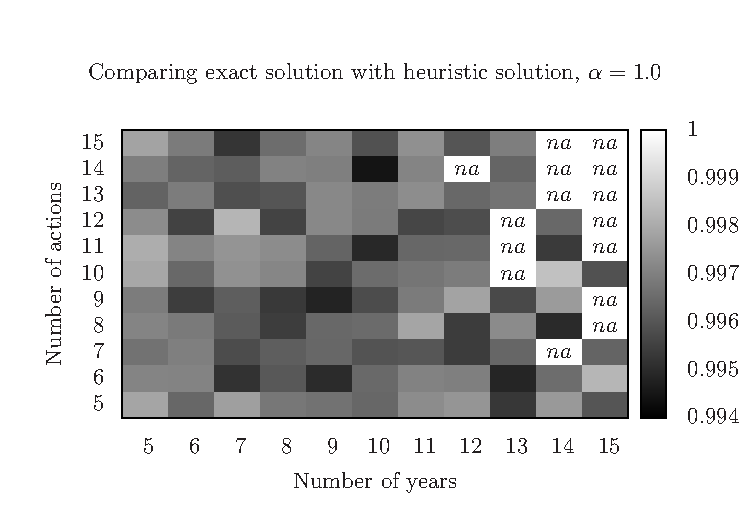
\includegraphics[scale=0.73, trim=1cm 0 0 0]{figs/comp_easy.pdf}
\caption{Comparison between the optimal solution (when available) 
and the solution by the meta-heuristics for $\alpha=1.0$.}
\label{fig:mh1_3}
\end{figure}
\todo[inline]{Discussion}

\begin{figure}
\centering
\missingfigure[figwidth=8cm]{}
\caption{Blah blah blah}
\label{fig:mh2_1}
\end{figure}

\begin{figure}
\centering
\missingfigure[figwidth=8cm]{}
\caption{Blah blah blah}
\label{fig:mh2_2}
\end{figure}

\begin{figure}
\centering
\missingfigure[figwidth=8cm]{}
\caption{Blah blah blah}
\label{fig:mh2_3}
\end{figure}

\todo[inline]{Discussion}

\subsection{Solution Analysis - All Instances}

In this subsection we compare the behavior of the meta heuristics in respect to one another,
considering all instances, we cannot compare the results with the optimal solution since it is unknown
for the larger instances.

Figures~\ref{fig:comp_1} to \ref{fig:comp_3} display the relative distance between the two proposed meta
heuristics considering the solution quality for the tree studied correlation values.

\begin{figure}
\centering
\missingfigure[figwidth=8cm]{}
\caption{Blah blah blah}
\label{fig:comp_1}
\end{figure}

\begin{figure}
\centering
\missingfigure[figwidth=8cm]{}
\caption{Blah blah blah}
\label{fig:comp_2}
\end{figure}

\begin{figure}
\centering
\missingfigure[figwidth=8cm]{}
\caption{Blah blah blah}
\label{fig:comp_3}
\end{figure}

\todo[inline]{Discussion}
